% Технологический раздел
\chapter{Технологический раздел}

В данном разделе описаны выбранные средства реализации базы данных и приложения, состав реализованной базы данных, ограничения целостности, роли базы данных, интерфейс доступа к данным и порядок тестирования функций базы данных.

\section{Средства реализации}

Для реализации базы данных выбрана СУБД PostgreSQL. Данная СУБД поддерживает ACID-транзакции, домены, перечислимые типы, индексы, триггеры, хранимые функции и процедуры, диапазонные типы данных, а также ограничение EXCLUDE. Эти возможности позволяют перенести критические правила предметной области на уровень базы данных: запрет пересечения записей по времени, проверку актуальности цены, пересчет состояния счета и контроль допустимых статусов.

PostgreSQL также подходит для выбранной предметной области за счет развитой поддержки внешних ключей, транзакционной согласованности и диапазонных типов данных~\cite{postgres_range}. Расширение btree\_gist используется для ограничения пересечения временных интервалов. Для генерации UUID применяется расширение pgcrypto.

Для серверной части выбраны язык Go~\cite{go_docs}, пакет database/sql, драйвер pgx и фреймворк Gin~\cite{gin_docs}. Такое сочетание позволяет реализовать REST API и разделить код backend-приложения на слои Handler, Service и Repository. При этом критическая бизнес-логика не дублируется в приложении, а вызывается через функции PostgreSQL.

В качестве программного интерфейса доступа к данным выбран стандартный интерфейс Go database/sql с драйвером pgx. Выбор обусловлен тем, что данный интерфейс соответствует стеку backend-приложения, поддерживает параметризованные SQL-запросы, транзакции, работу через пул соединений и прямой вызов функций PostgreSQL. Универсальные интерфейсы ODBC, ADO.NET и JDBC в данном проекте не выбраны, так как они ориентированы на другие технологические платформы или требуют лишнего промежуточного слоя. Полноценная ORM также не использована, поскольку в курсовой работе требуется явно показать работу с реализованными функциями, триггерами и ограничениями базы данных.

Для клиентской части выбраны React~\cite{react_docs} и TypeScript~\cite{typescript_docs}. Клиентское приложение используется как демонстрационный интерфейс для регистрации пациента, просмотра прайс-листа, просмотра расписания, записи на прием, отмены записи, проведения приема и регистрации оплаты.

Для кэширования часто запрашиваемых данных используется Redis~\cite{redis_docs}. В кэш помещаются актуальный прайс-лист услуг и представление расписания врача за выбранный интервал. Сводная информация о выбранных средствах приведена в таблице~\ref{tab:stack}.

\begin{table}[H]
    \centering
    \caption{Выбранные средства реализации}
    \label{tab:stack}
    \small
    \begin{tabularx}{\textwidth}{|>{\raggedright\arraybackslash}p{3.3cm}|>{\raggedright\arraybackslash}p{4.2cm}|>{\raggedright\arraybackslash}X|}
        \hline
        Слой & Технология & Назначение \tabularnewline
        \hline
        Frontend & React + TypeScript & Реализация пользовательского интерфейса \tabularnewline
        \hline
        Backend & Go + Gin & Реализация REST API и серверной логики \tabularnewline
        \hline
        Доступ к БД & database/sql + pgx & Выполнение SQL-запросов и вызов функций PostgreSQL \tabularnewline
        \hline
        СУБД & PostgreSQL & Хранение данных, контроль целостности, индексы, функции и триггеры \tabularnewline
        \hline
        InMemory СУБД & Redis & Кэширование прайс-листа и расписания врачей \tabularnewline
        \hline
        API & REST & Обмен данными между frontend и backend \tabularnewline
        \hline
    \end{tabularx}
\end{table}
\normalsize

\section{Состав реализованной базы данных}

База данных реализована в сценарии db/schema.sql. В ней созданы логические схемы security, catalog, medical, scheduling и billing. Такое разбиение отделяет учетные записи и роли от справочников, медицинских данных, расписания и финансового контура.

Состав реализованных таблиц приведен в таблице~\ref{tab:implemented-entities}.

\begin{table}[H]
    \centering
    \caption{Сущности реализованной базы данных}
    \label{tab:implemented-entities}
    \footnotesize
    \renewcommand{\arraystretch}{1.08}
    \begin{tabularx}{\textwidth}{|>{\raggedright\arraybackslash}p{3.5cm}|>{\raggedright\arraybackslash}X|}
        \hline
        Схема & Реализованные сущности \tabularnewline
        \hline
        security & roles, users, user\_roles. Сущности отвечают за учетные записи, прикладные роли и связь многие-ко-многим между пользователями и ролями. \tabularnewline
        \hline
        catalog & specialties, services, service\_prices, представление current\_price\_list. Сущности описывают специальности, услуги и историю цен. \tabularnewline
        \hline
        medical & patients, doctors, doctor\_services, visits, visit\_services. Сущности хранят данные пациентов, врачей, оказанных услуг и результатов приема. \tabularnewline
        \hline
        scheduling & doctor\_availability, doctor\_absences, appointments. Сущности реализуют расписание, периоды отсутствия врача и записи пациентов на прием. \tabularnewline
        \hline
        billing & invoices, invoice\_items, payments. Сущности отвечают за формирование счетов, строки счетов и регистрацию оплат. \tabularnewline
        \hline
    \end{tabularx}
\end{table}
\normalsize

Связи многие-ко-многим реализованы через отдельные промежуточные таблицы. В качестве первичных ключей основных сущностей используются UUID. Фрагмент реализации сущности записи на прием приведен в листинге~\ref{lst:appendix-appointments} приложения~А.

\section{Реализованные ограничения целостности}

В базе данных реализованы домены, перечислимые типы, первичные и внешние ключи, ограничения уникальности, проверки значений, диапазонные ограничения и индексы. Основные группы ограничений приведены в таблице~\ref{tab:implemented-constraints}.

\begin{table}[H]
    \centering
    \caption{Реализованные ограничения целостности}
    \label{tab:implemented-constraints}
    \footnotesize
    \renewcommand{\arraystretch}{1.1}
    \begin{tabularx}{\textwidth}{|>{\raggedright\arraybackslash}p{4.0cm}|>{\raggedright\arraybackslash}X|}
        \hline
        Группа ограничений & Реализация \tabularnewline
        \hline
        Форматы контактных данных & Домены security.email\_address и security.phone\_number проверяют формат e-mail и телефона. \tabularnewline
        \hline
        Состояния сущностей & Перечислимые типы user\_status, patient\_status, doctor\_status, service\_status, appointment\_status, invoice\_status, payment\_status. \tabularnewline
        \hline
        Ссылочная целостность & Внешние ключи связывают пользователей с ролями, врачей со специальностями, записи с пациентами и врачами, визиты с записями, счета с визитами, оплаты со счетами. \tabularnewline
        \hline
        Уникальность & Уникальны логины пользователей, коды ролей, коды услуг, названия специальностей, связь врача с учетной записью, связь визита с записью и связь счета с визитом. \tabularnewline
        \hline
        Числовые проверки & Ограничения CHECK запрещают отрицательные суммы, нулевое количество услуг, некорректную длительность приема и дату рождения позже текущей даты. \tabularnewline
        \hline
        Временные интервалы & Для цен, доступности, отсутствий и записей используются диапазоны TSTZRANGE; дополнительно проверяется, что окончание интервала позже начала. \tabularnewline
        \hline
        Запрет пересечений & Ограничения EXCLUDE запрещают пересечение периодов цен одной услуги, активных интервалов доступности врача и активных записей одного врача. \tabularnewline
        \hline
    \end{tabularx}
\end{table}
\normalsize

Для ускорения ключевых операций созданы индексы по статусам пользователей, пациентов, врачей и услуг, по телефону пациента, по специальности врача, по истории цен, по расписанию врача, по истории пациента, по счетам пациента и по оплатам счета. Фрагменты реализации ограничений целостности приведены в листинге~\ref{lst:appendix-constraints} приложения~А.

\section{Реализованные функции и триггеры}

На стороне базы данных реализованы функции, инкапсулирующие основные правила предметной области. Перечень функций и триггеров приведен в таблице~\ref{tab:implemented-db-functions}. Схемы алгоритмов данных функций и триггеров приведены в конструкторском разделе на рисунках~\ref{fig:yed-set-updated-at}--\ref{fig:design-refresh-invoice-triggers}.

\begin{table}[H]
    \centering
    \caption{Реализованные функции и триггеры базы данных}
    \label{tab:implemented-db-functions}
    \footnotesize
    \renewcommand{\arraystretch}{1.08}
    \begin{tabularx}{\textwidth}{|>{\raggedright\arraybackslash}p{4.4cm}|>{\raggedright\arraybackslash}X|}
        \hline
        Объект & Назначение \tabularnewline
        \hline
        \begin{tabular}[t]{@{}l@{}}security.\tabularnewline set\_updated\_at\end{tabular} & Обновляет поле updated\_at перед изменением записи. \tabularnewline
        \hline
        \begin{tabular}[t]{@{}l@{}}security.\tabularnewline has\_role\end{tabular} & Проверяет наличие прикладной роли у пользователя. \tabularnewline
        \hline
        \begin{tabular}[t]{@{}l@{}}catalog.\tabularnewline get\_service\_price\end{tabular} & Возвращает актуальную цену услуги на заданный момент времени. \tabularnewline
        \hline
        \begin{tabular}[t]{@{}l@{}}scheduling.\tabularnewline book\_appointment\end{tabular} & Создает запись на прием после проверки пациента, врача, услуги, доступности врача и отсутствия врача. \tabularnewline
        \hline
        \begin{tabular}[t]{@{}l@{}}scheduling.\tabularnewline cancel\_appointment\end{tabular} & Отменяет запись с учетом статуса записи и роли пользователя, инициировавшего отмену. \tabularnewline
        \hline
        \begin{tabular}[t]{@{}l@{}}medical.\tabularnewline complete\_visit\end{tabular} & Создает визит, фиксирует оказанные услуги, формирует счет и переводит запись в состояние completed. \tabularnewline
        \hline
        \begin{tabular}[t]{@{}l@{}}billing.\tabularnewline register\_payment\end{tabular} & Регистрирует оплату и инициирует пересчет состояния счета. \tabularnewline
        \hline
        \begin{tabular}[t]{@{}l@{}}billing.\tabularnewline refresh\_invoice\_state\end{tabular} & Пересчитывает итоговую сумму счета, сумму оплат и статус счета. \tabularnewline
        \hline
        trg\_\*\_updated\_at & Триггеры автоматического обновления поля updated\_at. \tabularnewline
        \hline
        \begin{tabular}[t]{@{}l@{}}trg\_invoice\_items\_\tabularnewline refresh\_invoice,\tabularnewline trg\_payments\_\tabularnewline refresh\_invoice\end{tabular} & Триггеры пересчета счета после изменения строк счета или оплат. \tabularnewline
        \hline
    \end{tabularx}
\end{table}
\normalsize

Реализация перечисленных объектов находится в сценарии db/schema.sql. Функции созданы операторами CREATE OR REPLACE FUNCTION, а автоматический вызов служебной логики обеспечивается триггерами CREATE TRIGGER. Функция получения актуальной цены услуги приведена в листинге~\ref{lst:appendix-get-service-price} приложения~А, фрагмент функции записи на прием -- в листинге~\ref{lst:appendix-book-appointment}, а триггеры пересчета состояния счета -- в листинге~\ref{lst:appendix-refresh-invoice-triggers}.

\section{Ролевая модель базы данных}

На уровне PostgreSQL реализованы три роли базы данных. Они отделяют владение схемой, работу backend-приложения и доступ к отчетным данным.

\begin{table}[H]
    \centering
    \caption{Ролевая модель на уровне базы данных}
    \label{tab:technology-db-roles}
    \footnotesize
    \renewcommand{\arraystretch}{1.08}
    \begin{tabularx}{\textwidth}{|>{\raggedright\arraybackslash}p{3.2cm}|>{\raggedright\arraybackslash}p{3.8cm}|>{\raggedright\arraybackslash}X|}
        \hline
        Роль & Назначение & Права \tabularnewline
        \hline
        clinic\_owner & Владелец структуры базы данных & Создание и изменение схем, таблиц, индексов, функций, триггеров и ролей. \tabularnewline
        \hline
        clinic\_api & Роль backend-приложения & USAGE на схемы, SELECT, INSERT, UPDATE, DELETE на таблицы, EXECUTE на функции. \tabularnewline
        \hline
        \begin{tabular}[t]{@{}l@{}}clinic\_\tabularnewline reporting\end{tabular} & Роль отчетов и аналитики & SELECT на таблицы и USAGE на схемы без прав изменения данных. \tabularnewline
        \hline
    \end{tabularx}
\end{table}
\normalsize

Прикладные роли пациента, администратора и врача хранятся в таблицах security.roles и security.user\_roles. Они используются backend-приложением и функцией has\_role для проверки бизнес-правил, например права администратора отменять запись без ограничения в 24 часа. Фрагмент SQL-сценария создания ролей и выдачи прав приведен в листинге~\ref{lst:appendix-db-roles} приложения~А.

\section{Разработка интерфейса доступа к базе данных}

Frontend не обращается к базе данных напрямую. Все операции выполняются через REST API backend-приложения. Backend-слой валидирует входные данные, вызывает репозитории и функции PostgreSQL, а затем возвращает результат клиенту в формате JSON.

Реализация доступа к данным построена по трехслойной схеме: Handler, Service и Repository. Обработчики HTTP-запросов отвечают за прием и валидацию DTO, сервисный слой выполняет прикладную координацию и работу с Redis-кэшем, а репозитории являются единственным слоем, напрямую выполняющим SQL-запросы через database/sql. Такой интерфейс отделяет клиентское приложение от конкретной СУБД и одновременно сохраняет явный доступ к функциям PostgreSQL, разработанным в рамках курсовой работы.

Компонентная структура приложения показана на рисунке~\ref{fig:technology-app-components}. Пользователь работает с React-интерфейсом, frontend отправляет REST-запросы в backend, а backend последовательно передает обработку на уровни Handler, Service и Repository. Репозиторий обращается к PostgreSQL как к основной СУБД и к Redis как к InMemory-хранилищу кэшируемых представлений.

\begin{figure}[H]
    \centering
    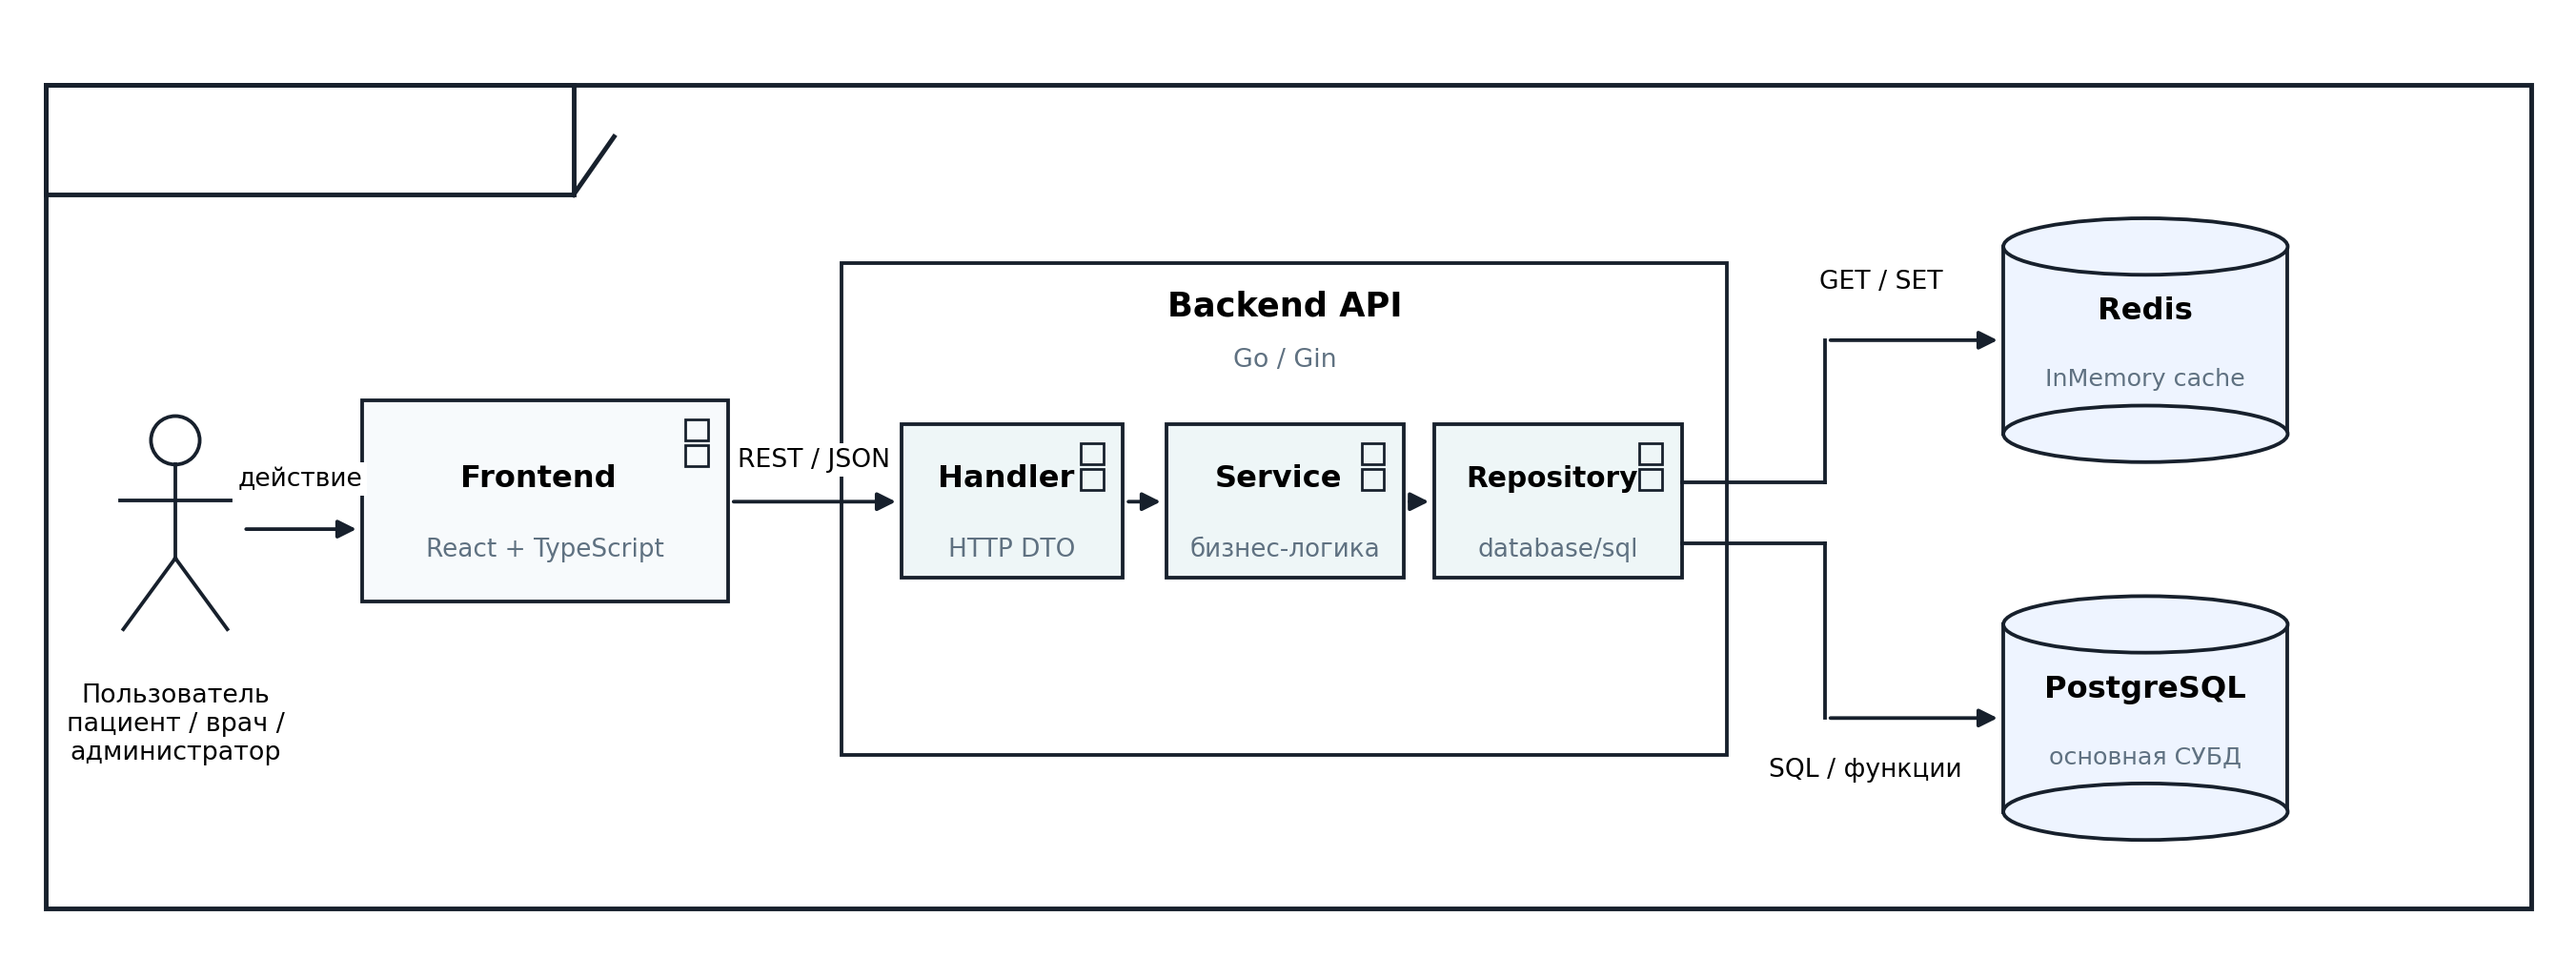
\includegraphics[width=\textwidth]{figures/technology_app_components.png}
    \caption{UML-диаграмма компонентов приложения}
    \label{fig:technology-app-components}
\end{figure}

Последовательность взаимодействия приложения с Redis и PostgreSQL при работе с кэшем показана на рисунке~\ref{fig:technology-cache-sequence}. На схеме отдельно приведены чтение данных через Redis-кэш и изменение данных с последующей инвалидацией кэша расписания. При отсутствии значения в Redis backend читает данные из PostgreSQL и сохраняет JSON-представление в кэш; при наличии значения результат возвращается без обращения к основной СУБД.

\begin{figure}[H]
    \centering
    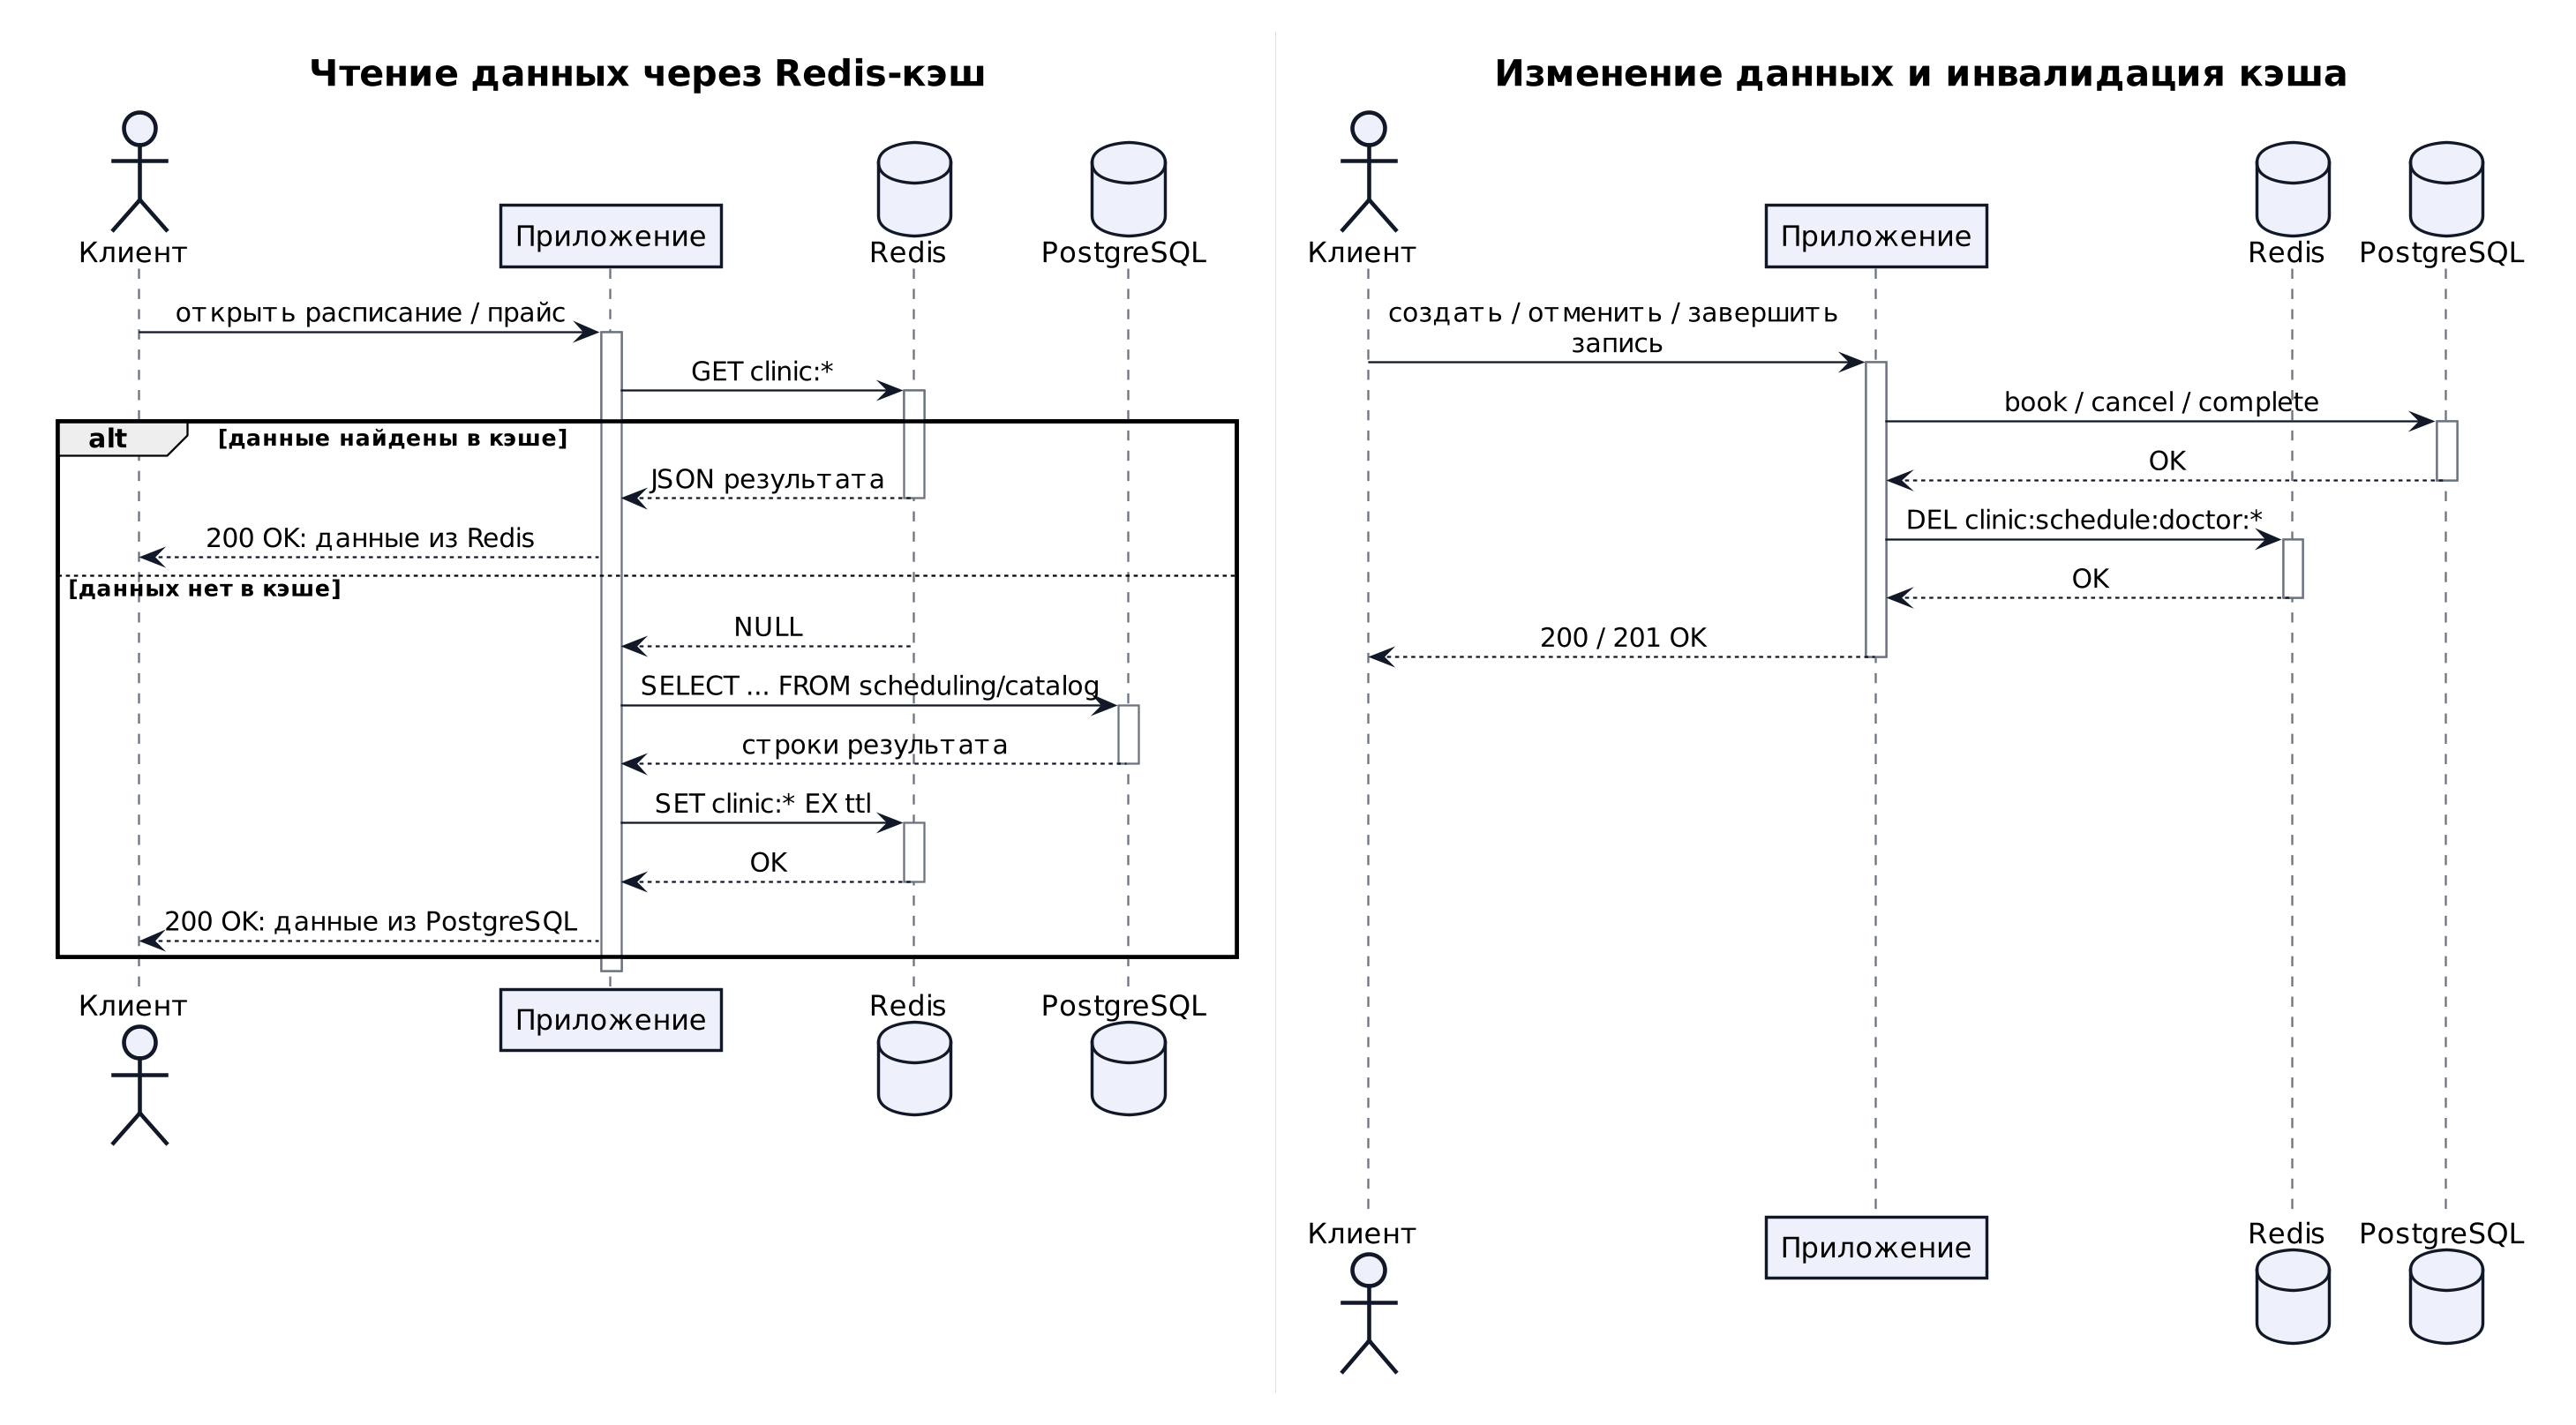
\includegraphics[width=\textwidth,height=0.82\textheight,keepaspectratio]{figures/technology_cache_sequence_plantuml_pair.png}
    \caption{UML-диаграмма последовательности доступа к PostgreSQL и Redis}
    \label{fig:technology-cache-sequence}
\end{figure}

\begin{table}[H]
    \centering
    \caption{Интерфейс доступа к базе данных}
    \label{tab:api-db-interface}
    \footnotesize
    \renewcommand{\arraystretch}{1.08}
    \begin{tabularx}{\textwidth}{|>{\raggedright\arraybackslash}p{4.4cm}|>{\raggedright\arraybackslash}p{4.2cm}|>{\raggedright\arraybackslash}X|}
        \hline
        Маршрут REST API & Обращение к базе данных & Назначение \tabularnewline
        \hline
        \begin{tabular}[t]{@{}l@{}}POST\tabularnewline /api/v1/patients\end{tabular} & medical.patients & Регистрация пациента. \tabularnewline
        \hline
        \begin{tabular}[t]{@{}l@{}}GET\tabularnewline /api/v1/services/\tabularnewline pricelist\end{tabular} & \begin{tabular}[t]{@{}l@{}}catalog.\tabularnewline current\_price\_list\end{tabular} & Получение актуального прайс-листа с использованием Redis-кэша. \tabularnewline
        \hline
        \begin{tabular}[t]{@{}l@{}}GET\tabularnewline /api/v1/doctors/\tabularnewline :doctorId/schedule\end{tabular} & \begin{tabular}[t]{@{}l@{}}doctor\_availability,\tabularnewline appointments\end{tabular} & Получение расписания врача с использованием Redis-кэша. \tabularnewline
        \hline
        \begin{tabular}[t]{@{}l@{}}POST\tabularnewline /api/v1/appointments\end{tabular} & \begin{tabular}[t]{@{}l@{}}scheduling.\tabularnewline book\_appointment\end{tabular} & Запись пациента на прием. \tabularnewline
        \hline
        \begin{tabular}[t]{@{}l@{}}POST\tabularnewline /api/v1/appointments/\tabularnewline :id/cancel\end{tabular} & \begin{tabular}[t]{@{}l@{}}scheduling.\tabularnewline cancel\_appointment\end{tabular} & Отмена записи. \tabularnewline
        \hline
        \begin{tabular}[t]{@{}l@{}}POST\tabularnewline /api/v1/appointments/\tabularnewline :id/complete\end{tabular} & \begin{tabular}[t]{@{}l@{}}medical.\tabularnewline complete\_visit\end{tabular} & Проведение приема и формирование счета. \tabularnewline
        \hline
        \begin{tabular}[t]{@{}l@{}}POST\tabularnewline /api/v1/invoices/\tabularnewline :id/payments\end{tabular} & \begin{tabular}[t]{@{}l@{}}billing.\tabularnewline register\_payment\end{tabular} & Регистрация оплаты по счету. \tabularnewline
        \hline
    \end{tabularx}
\end{table}
\normalsize

В рамках курсовой работы подготовлен frontend-интерфейс для выполнения основных операций медицинской клиники. Авторизация выполняется по учетной записи пользователя: после входа backend возвращает роль и связанные идентификаторы пациента или врача. Экран входа показан на рисунке~\ref{fig:frontend-login}. Рабочее место после входа адаптируется под роль пользователя и показано на рисунке~\ref{fig:frontend-workspace}. Оформление записи на прием приведено на рисунке~\ref{fig:frontend-workflow}.

\begin{figure}[H]
    \centering
    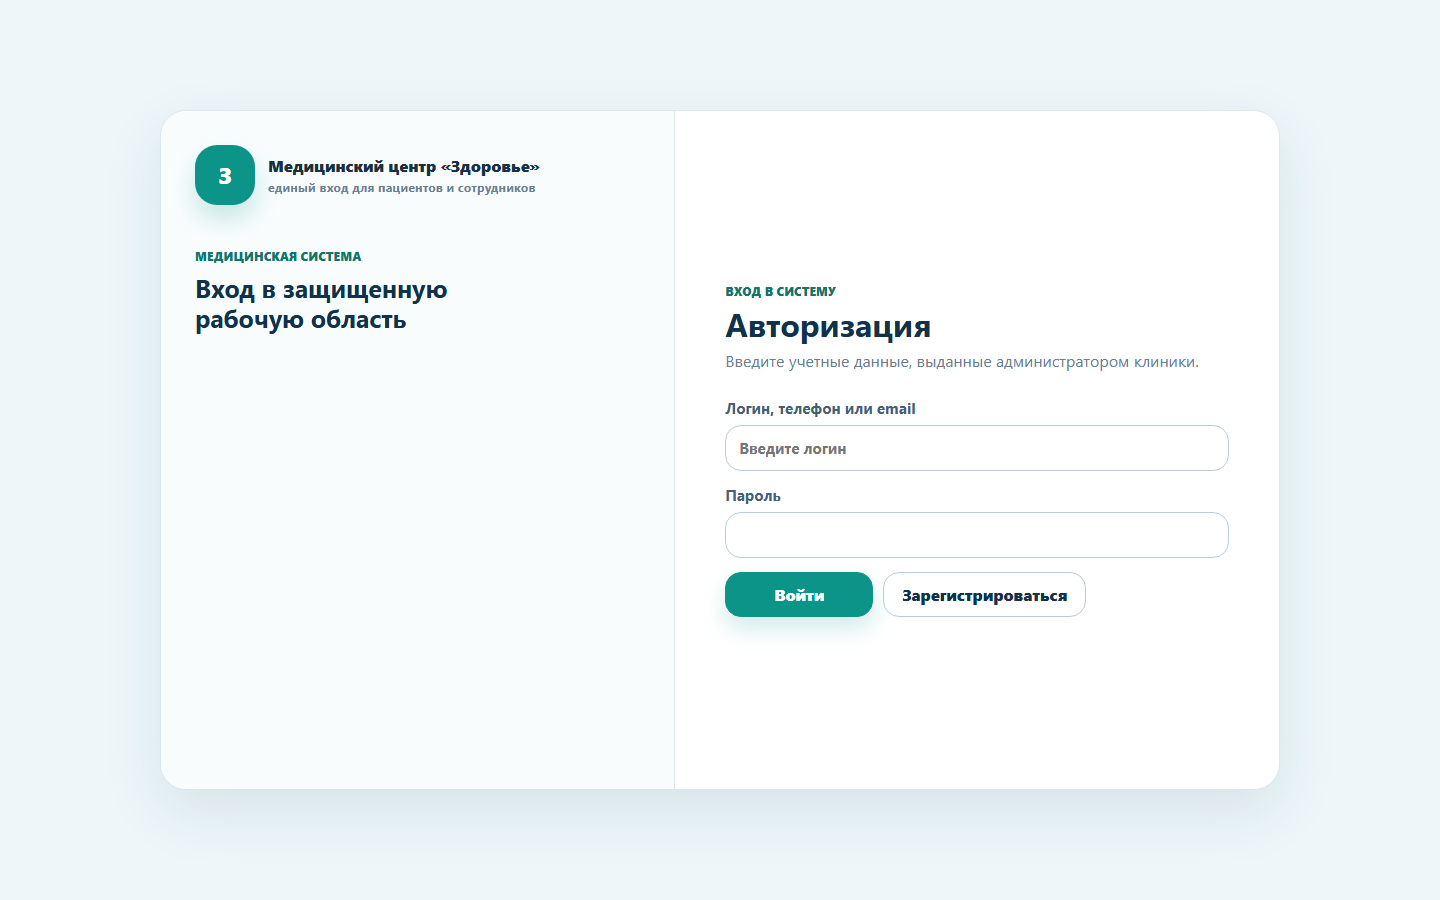
\includegraphics[width=\textwidth]{figures/frontend_login.png}
    \caption{Экран входа по пользователям}
    \label{fig:frontend-login}
\end{figure}

\begin{figure}[H]
    \centering
    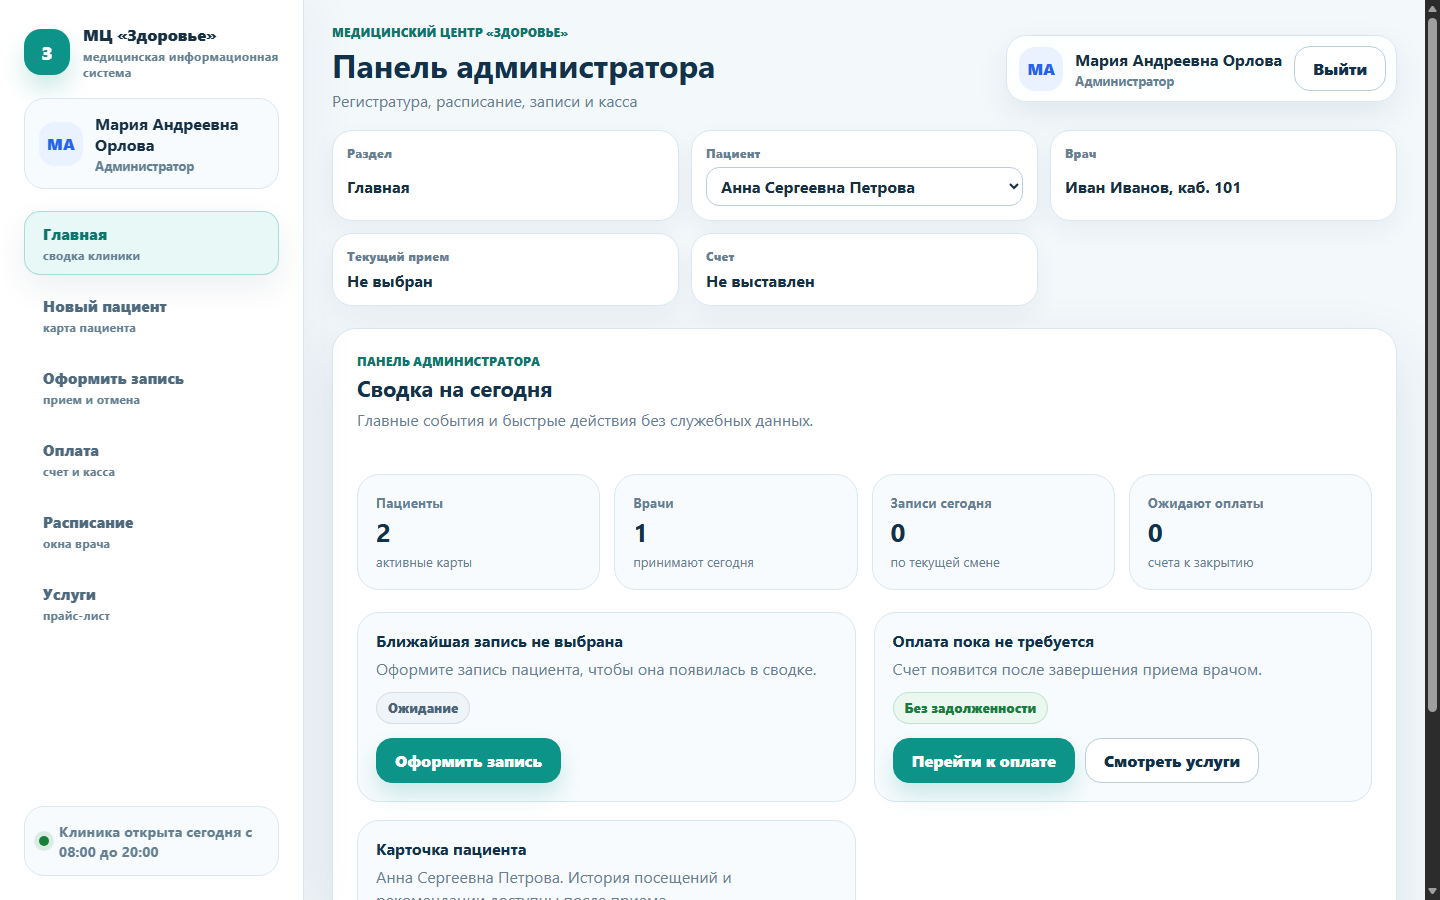
\includegraphics[width=\textwidth]{figures/frontend_role_workspace.png}
    \caption{Рабочее место пользователя после входа}
    \label{fig:frontend-workspace}
\end{figure}

\begin{figure}[H]
    \centering
    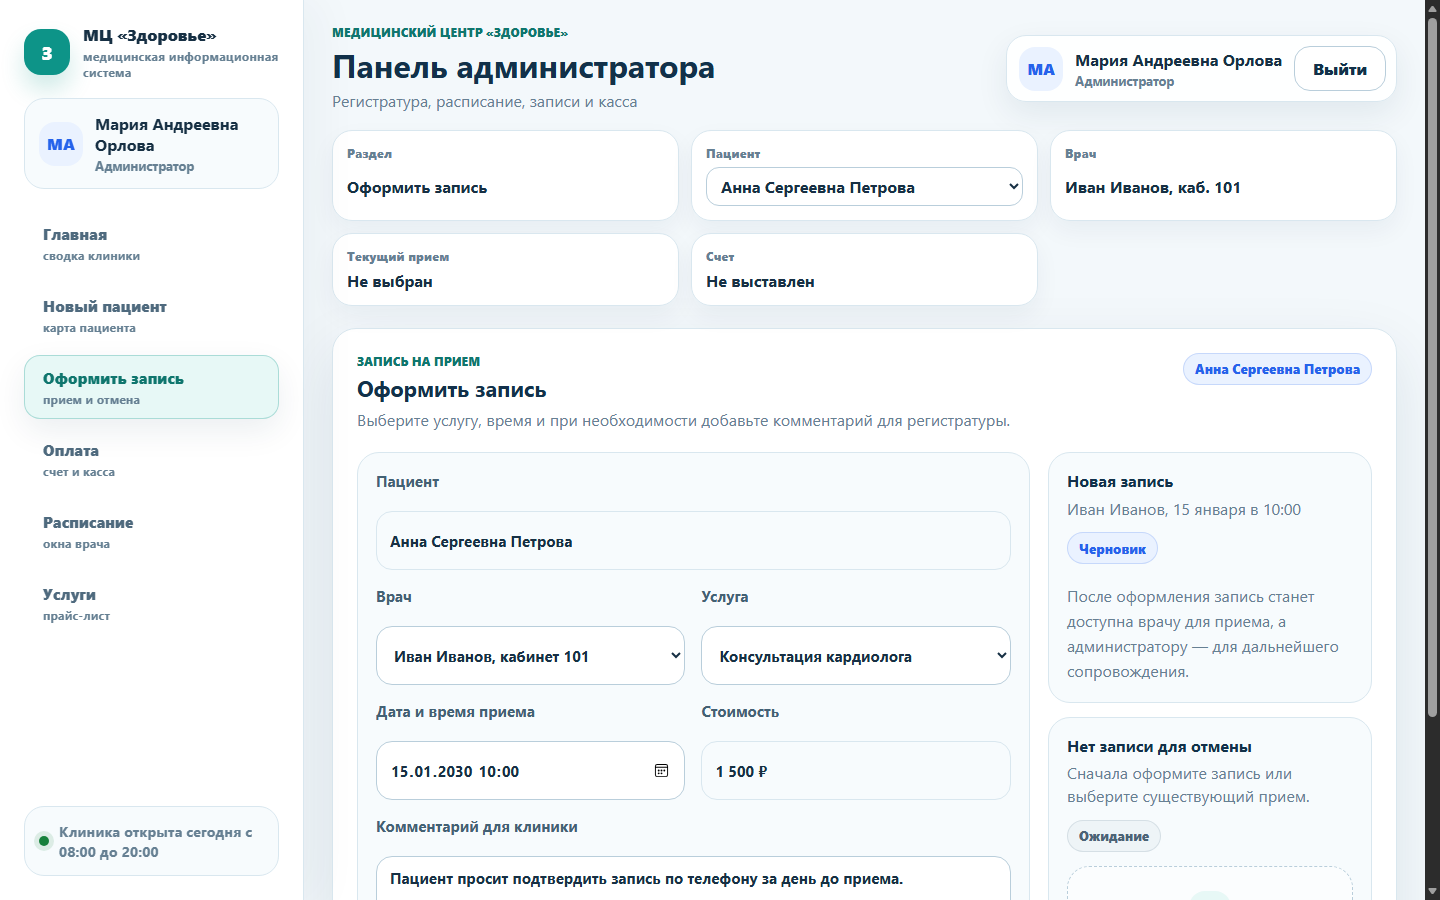
\includegraphics[width=\textwidth]{figures/frontend_workflow.png}
    \caption{Экран оформления записи на прием}
    \label{fig:frontend-workflow}
\end{figure}

Для входной валидации в Go используется пакет go-playground/validator. Входные UUID проверяются на ненулевое значение, телефон проверяется регулярным выражением, e-mail проверяется стандартным валидатором, а дата рождения передается типом, сериализуемым в формат YYYY-MM-DD. Фрагмент репозитория, вызывающего функции PostgreSQL через database/sql, приведен в листинге~\ref{lst:appendix-go-repository} приложения~А.

\section{Порядок тестирования и классы эквивалентности}

Тестирование выполнялось на трех уровнях: проверка входной валидации backend-приложения, проверка SQL-сценариев базы данных и проверка интеграционных сценариев через REST API. Для базы данных подготовлены сценарии функциональной проверки, конкурентного доступа и производительности.

Классы эквивалентности для функций базы данных приведены в таблице~\ref{tab:equivalence-classes}.

\begin{table}[H]
    \centering
    \caption{Классы эквивалентности для функций базы данных}
    \label{tab:equivalence-classes}
    \scriptsize
    \renewcommand{\arraystretch}{1.08}
    \begin{tabularx}{\textwidth}{|>{\raggedright\arraybackslash}p{3.5cm}|>{\raggedright\arraybackslash}X|>{\raggedright\arraybackslash}X|}
        \hline
        Функция & Корректные классы & Некорректные классы \tabularnewline
        \hline
        \begin{tabular}[t]{@{}l@{}}set\_\tabularnewline updated\_at\end{tabular} & Обновление строки таблицы, содержащей поле updated\_at. & Отсутствие поля updated\_at в таблице, к которой ошибочно подключен триггер. \tabularnewline
        \hline
        has\_role & Пользователь имеет требуемую роль; пользователь не имеет требуемую роль. & Несуществующий пользователь или несуществующий код роли. \tabularnewline
        \hline
        \begin{tabular}[t]{@{}l@{}}get\_service\_\tabularnewline price\end{tabular} & Для услуги найдена цена, действующая на заданный момент. & Услуга не имеет активной цены на заданный момент. \tabularnewline
        \hline
        \begin{tabular}[t]{@{}l@{}}book\_\tabularnewline appointment\end{tabular} & Активный пациент, активный врач, активная услуга, время в будущем, интервал входит в расписание и не пересекается с другой записью. & Прошедшее время, неактивный пациент, неактивный врач, услуга не закреплена за врачом, услуга неактивна, время вне расписания, отсутствие врача, пересечение с другой записью. \tabularnewline
        \hline
        \begin{tabular}[t]{@{}l@{}}cancel\_\tabularnewline appointment\end{tabular} & Отмена записи со статусом booked; отмена администратором; отмена пациентом более чем за 24 часа. & Несуществующая запись, статус не booked, отмена пациентом менее чем за 24 часа до приема. \tabularnewline
        \hline
        \begin{tabular}[t]{@{}l@{}}complete\_\tabularnewline visit\end{tabular} & Завершение записи врачом, связанным с приемом; завершение с базовой услугой; завершение с дополнительными оказанными услугами. & Несуществующая запись, другой врач, статус не booked, дополнительная услуга не закреплена за врачом. \tabularnewline
        \hline
        \begin{tabular}[t]{@{}l@{}}register\_\tabularnewline payment\end{tabular} & Регистрация оплаты с положительной суммой и допустимым способом оплаты. & Несуществующий счет, неположительная сумма, недопустимый способ оплаты. \tabularnewline
        \hline
        \begin{tabular}[t]{@{}l@{}}refresh\_\tabularnewline invoice\_state\end{tabular} & Нет оплат, частичная оплата, полная или избыточная оплата. & Несуществующий счет; некорректные строки счета невозможны при соблюдении ограничений CHECK. \tabularnewline
        \hline
        Триггеры пересчета счета & Добавление, изменение или удаление строки счета; добавление, изменение или удаление оплаты. & Ошибочная привязка триггера к таблице без поля invoice\_id. \tabularnewline
        \hline
    \end{tabularx}
\end{table}
\normalsize

Порядок проверки базы данных включает следующие шаги:
\begin{enumerate}
    \item создание структуры базы данных из сценария db/schema.sql;
    \item загрузку начальных данных из сценария db/seed.sql;
    \item выполнение сценария db/test\_scenarios.sql, проверяющего регистрацию пациента, валидацию e-mail и телефона, запись, запрет пересечения, отмену, проведение приема, формирование счета и оплату;
    \item выполнение двух сценариев конкурентного доступа:\\
    db/concurrency\_session\_1.sql;\\
    db/concurrency\_session\_2.sql;
    \item загрузку массового набора данных из db/bulk\_seed.sql и выполнение запросов EXPLAIN ANALYZE из db/performance.sql.
\end{enumerate}

Фрагмент сценария проверки некорректного класса эквивалентности для записи на прием приведен в листинге~\ref{lst:appendix-overlap-test} приложения~А.

На уровне backend выполняются unit-тесты валидаторов, обработки ошибок PostgreSQL, поведения кэша и HTTP-маршрутов. Для frontend выполняется сборка npm run build, подтверждающая корректность TypeScript-кода и клиентского интерфейса.

\section{Вывод}

В технологическом разделе обоснован выбор PostgreSQL, Redis, Go, Gin, React и TypeScript, описаны реализованные сущности, ограничения целостности, функции, триггеры, ролевая модель базы данных, REST-интерфейс доступа к данным и порядок тестирования. Реализация соответствует требованиям задания и использует возможности СУБД для контроля критических правил медицинской клиники.

\clearpage
